\documentclass[../main.tex]{subfiles}


\begin{document}

\section{Implementation}

Following the idea of our approach, we have implemented STCD. The source code is available at {\color{blue} \url{https://github.com/CSCC5704/SourceCodewithUI}}.

After catching all the tokens and accumulating their frequencies, in the pretreatment of variable names, we introduced bigram similarity. After actual testing, the threshold is set to 0.7 in our project. If the similarity of two variable names is higher than 0.7, then they are considered the same and their frequency will be compared.

For each category of tokens, to calculate the similarity, we used am algorithm similar to Levenshtein Distance:

\begin{equation}
\text{Sim}(\text{List}_x, \text{List}_y) = 1 - \frac{\sum \text{Diff}(\text{Elem}_{x_i}, \text{Elem}_{y_i})} {\sum (\text{Freq}_{x_i} + \text{Freq}_{y_i} )}
\end{equation}

where the difference is defined by:

\begin{equation}
\text{Diff}(\text{Elem}_{x_a}, \text{Elem}_{y_a}) = \text{Abs}(\text{Freq}_{x_a} - \text{Freq}_{y_a})
\end{equation}

This is a well-defined calculation, because no difference in the lists gives a similarity of 1, while totally different lists give similarity of 0.

An example shows the resonablity of this algorithm:

AN EXAMPLE GOES HERE

Before using machine learning to set the weights, we set the weights arbitrarily, which may not provide the best result, but it works in finding clones. 

To get training data, we use manual selection to find ``ground truth''. However it is not so easy to manually find ``ground truth'': if a Java file has 100 methods, then we need to compare $\frac{100\times 99}{2} = 4950$ pairs. In these pairs, most of them are not clone, so we applied our tool to the Java file, with a low threshold--0.65 to rule out most of the pairs, and manually checked the rest. This reduced our work from thousands of comparasions to less than a hundred. This process may introduce false negatives but we consider it to be small.

We selected training files from SWT--the tool to develop our UI. The advantage to use data from the same project is that machine learning can learn the developer's behavior. We chose 10 Java files, namely: \textit{Combo.java, DragSource.java, DropTarget.java, FormData.java, Label.java, Printer.java, Program.java, Shell.java, Text.java, WebKit.java}. The number of methods ranges from 12 to 125.

In the training process, MLP studies 50 clone pairs and 150 non-clone pairs to decide the best weights. There are much more non-clone pairs but studying more of them does not give a better result.

To make STCD more user friendly, we also developed a UI, as shown in Fig:\ref{fig:Graph_3}.

\begin{figure*}
\centering 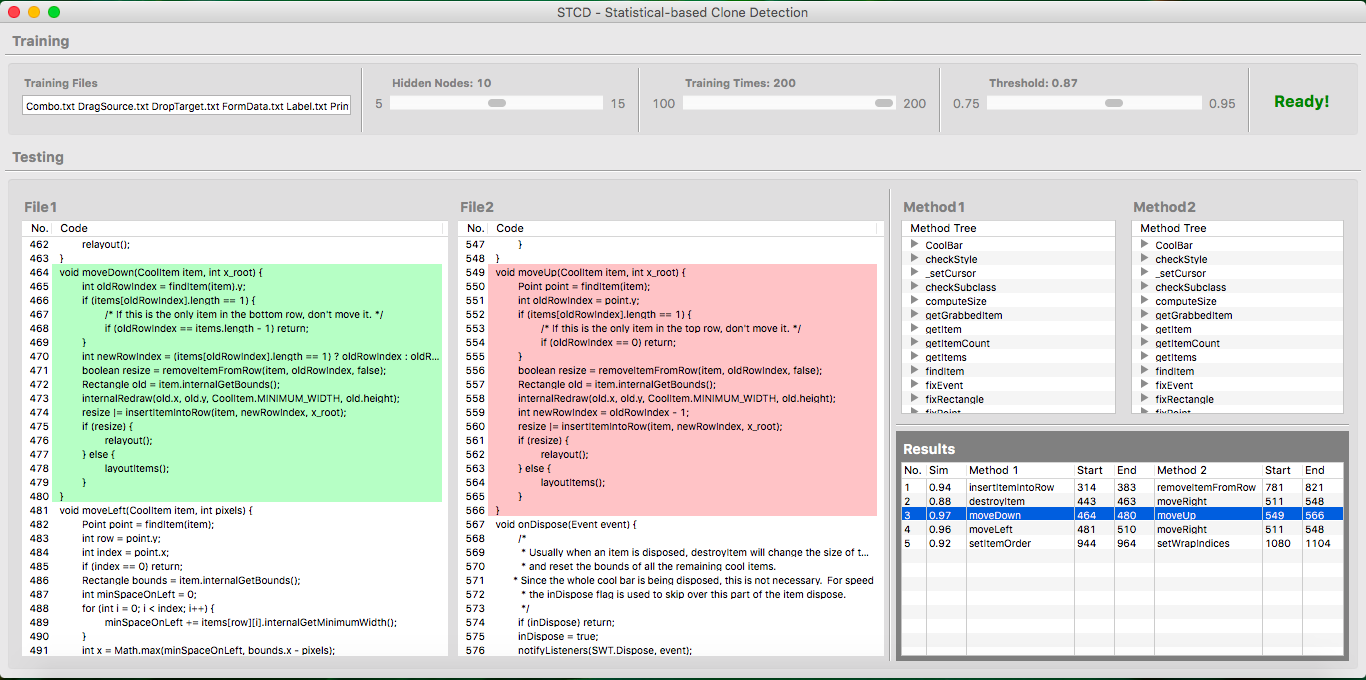
\includegraphics[width = \textwidth]{Graph_3} 
\caption{User Interface} \label{fig:Graph_3}
\end{figure*}

The instruction to use STCD:

\begin{enumerate}
\item From the training menu users are able to select training files. STCD can also run the testing without training, then starts from Step 4.
\item After the selection of training files, users can adjust Hidden Nodes and Training Times in the MLP training process, as well as the threshold. 
\item Run the training until it's ready, that takes less than seconds. 
\item From the test menu users can choose the Java file to test. A second file can be selected, if not, the test will be within the same file. 
\item Run the test until the result is shown.
\item From the Results window, click on the clone and the clone pairs will be shown in green and red color. The Method 1 and Method 2 windows show the token frequencies in each method.  
\end{enumerate}




\end{document}